\documentclass{article}
\usepackage{fouriernc}
%\usepackage[utf8]{vietnam}
\usepackage{amsmath,amssymb}
\usepackage{mathrsfs}
\usepackage{tikz,tkz-tab}
\usepackage[top=1.75cm, bottom=1.75cm, left=1.5cm, right=1.5cm] {geometry}
\usepackage{fancyhdr}
\usepackage[many]{tcolorbox}
\usepackage[dethi]{ex_test}
\newcommand{\name}[2]{
	%\newpage
	\setcounter{ex}{0}
	\begin{tcolorbox}[boxrule=1.5pt,arc=1mm,breakable,colframe=violet,colback=yellow!5]
		\begin{minipage}[t]{0.37\textwidth}
			\begin{center}
				\textcolor{violet}{\bf\fontfamily{qag}\selectfont#1}
			\end{center}
		\end{minipage}
		\begin{minipage}[t]{0.63\textwidth}
			\begin{center}
				\textcolor{violet}{\bfseries\fontfamily{qag}\selectfont #2}
			\end{center}
		\end{minipage}
	\end{tcolorbox}
}
\def\bbox{\begin{tcolorbox}[
		enhanced jigsaw,breakable,pad at break*=1mm,
		colback=gray!2, colframe=black,
		before skip=0mm,after skip=2mm,
		boxrule=1pt,drop fuzzy shadow=white!50!gray,
		left=1mm,right=1mm,top=1mm,bottom=0mm,
		sharp corners,
		rounded corners=northeast,
		arc is angular,arc=2mm,
		]
	}
	\def\ebox{\end{tcolorbox}}
\renewtheorem{ex}{\color{blue} Câu}
%\AtBeginEnvironment{ex}{%
%	\bbox
%	}
%\AtEndEnvironment{ex}{\ebox
%}
\AfterEndEnvironment{ex}{
		%\hspace{.45\textwidth}\textbf{Bài làm}\\ 
		\ifthenelse{\theex>38}{
		\foreach \i in {1,...,5}
		{\noindent\tikz\draw[gray,dash pattern=on 4pt off 1pt,ultra thin](0,0)--(.49\textwidth,0)(.51\textwidth,0)--(\textwidth,0)
		%(.5\textwidth,.45)--(.5\textwidth,-.05)
		;\\}
		}
		{\foreach \i in {1,...,2}
		%{\noindent\tikz\draw[dotted](-3,0)--(\linewidth,0);\\[2mm]}
		{\noindent\tikz\draw[gray,dash pattern=on 4pt off 1pt,ultra thin](0,0)--(.49\textwidth,0)(.51\textwidth,0)--(\textwidth,0)
		%(.5\textwidth,.45)--(.5\textwidth,-.05)
		;\\}
		}
}
\everymath{\displaystyle}
\def\hoac#1{\left[\begin{aligned}#1\end{aligned}\right.}
\def\heva#1{\left\{\begin{aligned}#1\end{aligned}\right.}
\def\vec#1{\overrightarrow{#1}}
\begin{document}
%\begin{name}
{Chuyên ngoại ngữ Hà Nội}
{ĐỀ THI THỬ TỐT NGHIỆP THPT--NĂM 2022 }
\end{name}
\Opensolutionfile{ans}[ngoaingu]
\begin{ex} %Câu 1
Cho cấp số nhân $( {{u}_{n}} )$ với ${{u}_{1}}=5$ và công bội $q=-2$. Giá trị của ${{u}_{2}}$ bằng 
\choice 
{ $7$}
{ \True $-10$}
{ $3$}
{ $-\dfrac{5}{2}$} \end{ex} 
\begin{ex} %Câu 2
Trong không gian $Oxyz$, đường thẳng $\Delta:\heva{
& x=2+2t \\ 
& y=-1+3t \\ 
& z=-4+3t \\ 
}$ đi qua điểm nào dưới đây? 
\choice 
{  $P( 4;2;1 )$}
{ $Q( -2;-7;10 )$} 
{ $N( 0;-4;7 )$}
{ \True $M( 0;-4;-7 )$} \end{ex} 
\begin{ex} %Câu 3
Cho hình chóp $S.ABCD$ có đáy $ABCD$ là hình vuông cạnh $a$. Đường thẳng $SA$ vuông góc với mặt phẳng đáy, $SA=a$. Gọi $E$ là trung điểm của $CD$. Khoảng cách từ $E$ đến mặt phẳng $( SAB )$ bằng
\choice 
{ $\dfrac{a\sqrt{2}}{2}$}
{ \True $a$}
{ $a\sqrt{2}$}
{ $2a$} \end{ex} 
\begin{ex} %Câu 4
Họ nguyên hàm của hàm số $f( x )={{5}^{x}}$ là
\choice 
{ \True $\int {f(x) \mathrm{d} x}=\dfrac{{{5}^{x}}}{\ln 5}+C$}
{ $\int {f( x ) \mathrm{d} x}={{5}^{x}}\ln 5+C$} 
{ $\int {f( x ) \mathrm{d} x}={{5}^{x+1}}+C$}
{ $\int {f( x ) \mathrm{d} x}=\dfrac{5^{x+1}}{x+1}+C$} 
\end{ex} 
\begin{ex} %Câu 5
Với mọi $a;b$ thỏa mãn $3\log a+2\log b=1$, khẳng định nào dưới đây đúng? 
\choice 
{ ${{a}^3}+b^2=1$}
{ \True ${{a}^3}b^2=10$}
{ $3a+2b=10$}
{ ${{a}^3}+b^2=10$} \end{ex} 
\begin{ex} %Câu 6
\immini[thm]{Hàm số nào có đồ thị là đường cong trong hình vẽ bên dưới?
\choice 
{ \True $y=x^4-4x^2+1$}
{ $y=\dfrac{x+1}{x-2}$}
{ $y=x^3+4x^2+1$}
{ $y=2x^2+1$} 
}{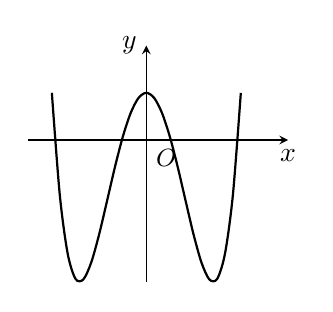
\begin{tikzpicture}[scale=.6]
\draw[-stealth] (-2.5,0) -- (3,0) node[below]{$x$};
\draw[-stealth] (0,-3) -- (0,2) node[left]{$y$};
\draw (0,0) node[below right]{\small $O$};
\draw[thick,smooth] plot[domain=-2:2](\x,{(\x)^4-4*(\x)^2+1});
\end{tikzpicture}}
\end{ex} 
\begin{ex} %Câu 7
Tập xác định của hàm số $y={{( x+2 )}^{\sqrt{2}}}$ là
\choice 
{ $\mathbb{R}\backslash \left\{ -2 \right\}$}
{ \True $( -2;+\infty )$}
{ $( 0;+\infty )$}
{ $\mathbb{R}$} \end{ex} 
\begin{ex} %Câu 8
Diện tích $S$ của mặt cầu bán kính $R$ được tính theo công thức nào dưới đây?
\choice 
{ $\dfrac{3}{4}\pi {{R}^2}$ }
{ $\pi {{R}^2}$ }
{ \True $4\pi {{R}^2}$ }
{ $\dfrac{4}{3}\pi {{R}^3}$ } \end{ex} 
\begin{ex} %Câu 9
Trên mặt phẳng tọa độ, cho $M( 4;-3 )$ là điểm biểu diễn của số phức $z$. Phần ảo của $z$ bằng
\choice 
{ $4$ }
{ $-3i$}
{ $-4$}
{ \True $-3$} \end{ex} 
\begin{ex} %Câu 10
Trong không gian $Oxyz$, cho tam giác $ABC$ có $A(-1;3;2)$, $B(2;0;5)$ và $C(0;-2;1)$. Đường trung tuyến $AM$ của tam giác $ABC$ có phương trình là
\choice 
{ \True $\dfrac{x+1}{2}=\dfrac{y-3}{-4}=\dfrac{z-2}{1}$}
{ $\dfrac{x-1}{2}=\dfrac{y+3}{-4}=\dfrac{z+2}{1}$} 
{ $\dfrac{x+1}{-2}=\dfrac{y-3}{-2}=\dfrac{z-2}{-4}$}
{ $\dfrac{x-1}{-2}=\dfrac{y+3}{-2}=\dfrac{z+2}{-4}$} \end{ex} 
\begin{ex} %Câu 11
Nếu $\int\limits_0^4{f(x)}\,\mathrm{d} x=37$ thì $\int\limits_0^4{[ 2f(x)-3x^2 ]}\,\mathrm{d} x$ bằng
\choice 
{ 12}
{ 18}
{ $-27$}
{ \True 10} \end{ex} 
\begin{ex} %Câu 12
Cho số phức $z$ thoả mãn: $(3+2i)\bar{z}+{{(2-i)}^2}=4+i$. Tổng phần thực và phần ảo của số phức $z$ bằng
\choice 
{ 3}
{ \True 0}
{ 2}
{ 1} \end{ex} 
\begin{ex} %Câu 13
Tiệm cận ngang của đồ thị hàm số $y=\dfrac{2x+1}{x-1}$ là đường thẳng có phương trình
\choice 
{ $x=2$}
{ $y=-2$}
{ $x=1$}
{ \True $y=2$} \end{ex} 
\begin{ex} %Câu 14
Tập nghiệm của bất phương trình ${{3}^{x}}\ge 12$ là
\choice 
{ $[ 4;\,+\infty )$}
{ $( -\infty;\,4 ]$}
{ \True $[ {{\log }_{3}}12;\,+\infty )$}
{ $( -\infty;\,{{\log }_{3}}12 ]$} \end{ex} 
\begin{ex} %Câu 15
Mô đun của số phức $z=4-3i$ bằng'
\choice 
{ \True $| z |=5$}
{ $| z |=7$}
{ $| z |=\sqrt{7}$}
{ $| z |=25$} \end{ex} 
\begin{ex} %Câu 16
Cho hình chóp $S.ABCD$ có tất cả các cạnh đều bằng $a$. Gọi $I$ và $J$ lần lượt là trung điểm của $SC$ và $BC$. Góc giữa hai đường thẳng $IJ$ và $SC$ bằng
\choice 
{ \True $60{}^\circ $}
{ $45{}^\circ $}
{ $90{}^\circ $}
{ $30{}^\circ $} \end{ex} 
\begin{ex} %Câu 17
Cho số phức $z=-3+4i$, khi đó $3z$ bằng 
\choice 
{ \True $z=-9+12i$}
{ $z=-3+12i$}
{ $z=9-12i$}
{ $z=-9+4i$} \end{ex} 
\begin{ex} %Câu 18
Nếu $\int\limits_{2}^5{f( x )\mathrm{d} x}=3$ và $\int\limits_{5}^{7}{f( x )\mathrm{d} x}=9$ thì $\int\limits_{2}^{7}{f( x )\mathrm{d} x}$ bằng
\choice 
{ $6$}
{ $3$}
{ $-6$}
{ \True $12$} \end{ex} 
\begin{ex} %Câu 19
Hàm số nào sau đây đồng biến trên $\mathbb{R}$?
\choice 
{ $y=x+\dfrac{1}{x+3}$}
{ $y=\dfrac{1}{x-2}$} 
{ \True $y=x^3-3x^2+3x+5$}
{ $y=x^4+x^2+1$} \end{ex} 
\begin{ex} %Câu 20
Trong không gian $Oxyz$, cho hai vectơ $\vec{u}=( -1;3;2 )$ và $\vec{v}=( -3;-1;2 )$. Khi đó $\vec{u}.\vec{v}$ bằng
\choice 
{ $3$ }
{ $2$}
{ $10$}
{ \True $4$} \end{ex} 
\begin{ex} %Câu 21
Cho khối lăng trụ đứng có cạnh bên bằng $5$, đáy là hình vuông có cạnh bằng $4$. Thể tích khối lăng trụ đã cho bằng
\choice 
{ $64$ }
{ $20$}
{ $100$}
{ \True $80$} \end{ex} 
\begin{ex} %Câu 22
Trên đoạn $[ -4;\,-1 ]$, hàm số $y=x+\dfrac{9}{x-1}$ đạt giá trị lớn nhất bằng
\choice 
{ \True $-5$}
{ $-\dfrac{29}{5}$}
{ $-\dfrac{11}{2}$}
{ $4$} \end{ex} 
\begin{ex} %Câu 23
Một tổ có 7 nam và 3 nữ. Chọn ngẫu nhiên đồng thời 2 người. Xác suất để 2 người được chọn có ít nhất một nữ bằng
\choice 
{ \True $\dfrac{8}{15}$}
{ $\dfrac{7}{15}$}
{ $\dfrac{1}{15}$}
{ $\dfrac{2}{15}$} \end{ex} 
\begin{ex} %Câu 24
Với mọi số thực $a$ dương khác 1, ${{\log }_{a}}\sqrt[3]{a}$ bằng
\choice 
{ \True $\dfrac{1}{3}$}
{ $3$}
{ $-3$}
{ $0$} \end{ex} 
\begin{ex} %Câu 25
Nếu $\int\limits_{3}^4{f( x )\mathrm{d} x}=3$ thì $\int\limits_{3}^4{-4f( x )\mathrm{d} x}$ bằng
\choice 
{ \True $-12$}
{ $-4$}
{ $12$}
{ $3$} \end{ex} 
\begin{ex} %Câu 26
Trong không gian $Oxyz$, cho điểm $M( -2;1;-1 )$ và đường thẳng $d:\dfrac{x-1}{-3}=\dfrac{y}{2}=\dfrac{z+1}{1}$. Mặt phẳng đi qua $M$ và vuông góc với $d$ có phương trình là
\choice 
{ \True $3x-2y-z+7=0$}
{ $-2x+y-z+7=0$} 
{ $3x-2y-z-7=0$}
{ $-2x+y-z-7=0$} \end{ex} 
\begin{ex} %Câu 27
Cho hàm số $f( x )=x+\cos x$. Khẳng định nào dưới đây là đúng?
\choice 
{ $\int{f( x )\mathrm{d} x}=x\sin x+\cos x+C$}
{ $\int{f( x )\mathrm{d} x}=1-\sin x+C$}
{ \True $\int{f( x )\mathrm{d} x}=\dfrac{x^2}{2}+\sin x+C$}
{ $\int{f( x )\mathrm{d} x}=\dfrac{x^2}{2}-\sin x+C$} 
\end{ex} 
\begin{ex} %Câu 28
Cho khối nón có đường cao $h$ và bán kính đáy $r$. Thể tích của khối nón đã cho được tính bởi công thức nào dưới đây?
\choice 
{ \True $V=\dfrac{1}{3}\pi {{r}^2}h$}
{ $V=\pi {{r}^2}h$}
{ $V=\pi r\sqrt{{{h}^2}+{{r}^2}}$}
{ $V=2\pi r\sqrt{{{h}^2}+{{r}^2}}$} \end{ex} 
\begin{ex} %Câu 29
\immini[thm]{Cho hàm số $y=f( x )$ xác định và liên tục trên đoạn $[ -2\,;\,2 ]$ và có đồ thị là đường cong trong hình vẽ sau. Điểm cực tiểu của đồ thị hàm số $y=f( x )$ là
\choice 
{ $x=1$}
{ $x=-2$}
{ \True $M( 1\,;\,-2 )$}
{ $M( -2\,;\,-4 )$} 
}{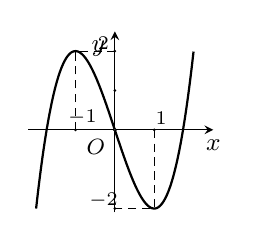
\begin{tikzpicture}[scale=.5]
\draw[-stealth] (-2.2,0) -- (2.5,0) node[below]{\small $x$};
\draw[-stealth] (0,-2.1) -- (0,2.5) node[below left]{\small $y$};
\draw [thin,densely dashed] (-1,0)|-(0,2)  (1,0)|-(0,-2) ;
\draw[thick,smooth,samples=100] plot[domain=-2:2](\x,{(\x)^3-3*(\x)});
\draw [fill=white,draw=black] (0,0) circle (1pt)node[below left]{\footnotesize $O$};
\foreach \x in{-1,1}\draw(\x,0) circle (.5pt) node[shift={(60:5pt)}]{\scriptsize $\x$};
\foreach \y in{-2,2,}\draw(0,\y) circle (.5pt) node[shift={(145:5pt)}]{\scriptsize $\y$};
\end{tikzpicture}}
\end{ex} 
\begin{ex} %Câu 30
Trong không gian $Oxyz$, mặt cầu $( S ):{{( x+1 )}^2}+{{( y-3 )}^2}+{{( z-2 )}^2}=16$ có tâm và bán kính là 
\choice 
{ $I( 1\,;\,-3\,;\,-2 )$ và $R=4$}
{ \True $I( -1\,;\,3\,;\,2 )$ và $R=4$} 
{ $I( 1\,;\,-3\,;\,-2 )$ và $R=16$}
{ $I( -1\,;\,3\,;\,2 )$ và $R=16$} \end{ex} 
\begin{ex} %Câu 31
Nghiệm của phương trình ${{\log }_{3}}( x-2 )=4$ là
\choice 
{ $x=79$}
{ $x=81$}
{ $x=66$}
{ \True $x=83$} \end{ex} 
\begin{ex} %Câu 32
Với $k;n$ là các số nguyên thỏa mãn $0\le k\le n$, công thức nào dưới đây đúng?
\choice 
{ $A_{n}^{k}=\dfrac{n!}{k!( n+k )!}$}
{ \True $A_{n}^{k}=\dfrac{n!}{( n-k )!}$} 
{ $A_{n}^{k}=\dfrac{n!}{k!( n-k )!}$}
{ $A_{n}^{k}=\dfrac{n!}{( n+k )!}$} \end{ex} 
\begin{ex} %Câu 33
Cho khối chóp có diện tích đáy $B$ và chiều cao $h$. Thể tích $V$ của khối chóp đã cho được tính theo công thức vào dưới đây?
\choice 
{ $V=\dfrac{1}{2}Bh$}
{ \True $V=\dfrac{1}{3}Bh$}
{ $V=\dfrac{4}{3}Bh$}
{ $V=Bh$} \end{ex} 
\begin{ex} %Câu 34
Trong không gian $Oxyz$, mặt phẳng $( P ):2x+y-1=0$ có một vectơ pháp tuyến là
\choice 
{ ${{\vec{n}}_{3}}=( 1;2;0 )$}
{ ${{\vec{n}}_{2}}=( 2;1;-1 )$}
{ ${{\vec{n}}_{1}}=( -2;-1;1 )$}
{ \True ${{\vec{n}}_{4}}=( 2;1;0 )$} \end{ex} 
\begin{ex} %Câu 35
Điểm nào sau đây thuộc đồ thị của hàm số $y=x^4-3x^2-5$?
\choice 
{ \True $N( 2;-1 )$}
{  $P( 1;3 )$}
{  $Q( -2;-9 )$}
{  $M( -1;-3 )$} \end{ex} 
\begin{ex} %Câu 36
Đạo hàm của hàm số $y={e^{3x}}$ là
\choice 
{ ${y}'={e^{3x}}$}
{ ${y}'={e^{3x}}.\ln 3$}
{ \True ${y}'=3{e^{3x}}$}
{ ${y}'=\dfrac{{e^{3x}}}{3}$} \end{ex} 
\begin{ex} %Câu 37
Cho hàm số $y=f( x )$ liên tục trên $\mathbb{R}$ và có bảng xét dấu của đạo hàm như sau:
 \\ \centerline{
\begin{tikzpicture}
\tkzTabInit[nocadre,lgt=1.2,espcl=2.2]
{$x$ /.6,$f'(x)$ /.6}
{$-\infty$,$-1$,$0$,$2$,$4$,$+\infty$}
\tkzTabLine{,+,$0$,-,d,+,$0$,-,$0$,+,}
\end{tikzpicture}
}\\
Số điểm cực trị của hàm số đã cho là
\choice 
{ $1$}
{ \True $4$}
{ $3$}
{ $2$} \end{ex} 
\begin{ex} %Câu 38
Cho hàm số $y=f( x )$ có bảng biến thiên như sau:
 \\ \centerline{
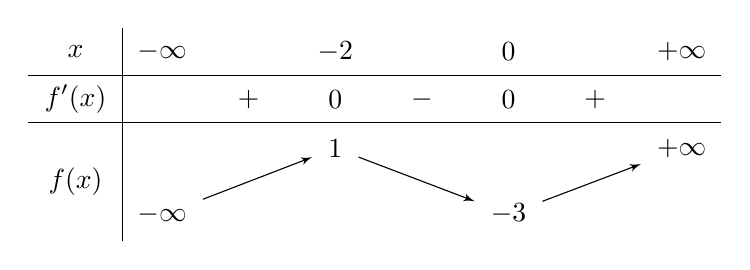
\begin{tikzpicture}
\tkzTabInit[nocadre,lgt=1.2,espcl=2.2]
{$x$ /.6,$f'(x)$ /.6,$f(x)$ /1.5}
{$-\infty$,$-2$,$0$,$+\infty$}
\tkzTabLine{,+,$0$,-,$0$,+,}
\tkzTabVar{-/ $-\infty$ ,+/$1$,-/$-3$,+/$+\infty$}
\end{tikzpicture}
}\\
Hàm số đã cho nghịch biến trên khoảng nào dưới đây?
\choice 
{ $( 0;\,+\infty )$}
{ $( -\infty;\,-2 )$}
{ $( -3;\,1 )$}
{ \True $( -2;\,0 )$} \end{ex} 
\begin{ex} %Câu 39
Cho ${{z}_{1}},\,\,{{z}_{2}}$ là hai nghiệm phức của phương trình $3{{z}^2}-7z+27=0$. Giá trị của ${{z}_{1}}|{{z}_{2}} |+{{z}_{2}}| {{z}_{1}}|$bằng 
\choice 
{ $3$}
{ \True $7$}
{ $6$}
{ $9$} \end{ex} 
\begin{ex} %Câu 40
Cho hàm số $y=f( x )$ có đạo hàm $f'( x )=12x^2-2,\,\,\forall x\in \mathbb{R}$. Biết $F( x )$ là một nguyên hàm của $f( x )$ thỏa mãn $F( 0 )=1$ và $F( 1 )=-1$, khi đó $f( 2 )$ bằng 
\choice 
{ $30$}
{ $36$}
{ $-3$}
{ \True $26$} \end{ex} 

\begin{ex} %Câu 42
Trong không gian $Oxyz,$ cho điểm $A( 2;-3;4 )$ và mặt phẳng $( P ):-x+2y+z=0$. Đường thẳng đi qua $A,$ cắt trục $Ox$ và song song với $( P )$ có phương trình là:
\choice 
{ $\dfrac{x-2}{1}=\dfrac{y+3}{2}=\dfrac{z-4}{-3}$}
{ \True $\dfrac{x-2}{2}=\dfrac{y+3}{3}=\dfrac{z-4}{-4}$} 
{ $\dfrac{x}{-2}=\dfrac{y+3}{-3}=\dfrac{z}{4}$}
{ $\dfrac{x+2}{1}=\dfrac{y+11}{2}=\dfrac{z-16}{-3}$} \end{ex} 
\begin{ex} %Câu 43
Cho khối chóp đều $S.ABCD$ có đáy $ABCD$ là hình vuông cạnh $a$. Biết diện tích tam giác $SAC$ là $\sqrt{2}a^2$, thể tích của khối chóp đã cho bằng
\choice 
{ \True $\frac{2}{3} a^{3}$ }
{ $a^{3}$ }
{ $2 \sqrt{2} a^{3}$ }
{ $\frac{4}{3} a^{3}$ } \end{ex} 
\begin{ex} %Câu 44
Cho khối nón đỉnh $S$ có bán kính đáy bằng $\sqrt{3}a $ . Gọi$M$ và $N$ là hai điểm thuộc đường tròn đáy sao cho $MN=2a$. Biết thể tích của khối nón là $\sqrt{2}\pi a^3$ , khoảng cách từ tâm của đường tròn đáy đến mặt phẳng $SMN$  là
\choice 
{ $\dfrac{a}{\sqrt{2}}$ }
{ $2a$ }
{ \True $a$ }
{ $\sqrt{3}a$ } \end{ex} 
\begin{ex} %Câu 45
Có bao nhiêu số nguyên $x$  thỏa mãn $\frac{\sqrt{3-{{\log }_{4}}\left( 2x \right)}}{-{{9}^{x}}+{{10.3}^{x+2}}-729}\le 0$?
\choice 
{ $31$ }
{ \True $29$ }
{ $27$ }
{$28$  }
 \end{ex} 
\begin{ex} %Câu 46
Cho hàm số $f(x)=3x^4+ax^3+bx^2+cx+d$  có ba điểm cực trị là $-2,1,2$. Gọi $y=g(x)$  là hàm số bậc hai có đồ thị đi qua ba điểm cực trị của đồ thị hàm số $y=f(x)$ . Diện tích hình phẳng giới hạn bởi hai đường $y=f(x)$  và $y=g(x)$  có giá trị thuộc khoảng
\choice 
{ $(34;35 )$ }
{ $(36;37 )$ }
{ \True $(37;38 )$ }
{ $(35;36 )$ } \end{ex} 
\Closesolutionfile{ans}
%\begin{name}
{Sở GD Hà Nam}
{ĐỀ THI THỬ TỐT NGHIỆP THPT--NĂM 2022 }
\end{name}
\Opensolutionfile{ans}[hanam]
\begin{ex} %{Cau 1}
Tập nghiệm của bất phương trinh $3^{x}<2$ lả.
\choice
{$\left(-\infty ; \log _{2} 3\right)$}
{\True $\left(-\infty ; \log _{3} 2\right)$}
{$\left(\log _{2} 3 ;+\infty\right)$}
{$\left(\log _{3} 2 ;+\infty\right)$}
\end{ex}

\begin{ex} %{Cau 2}
Cho khối chóp có diện tích đáy $B$ và chiều cao $h$. Thế tich $V$ của khối chóp đã cho được tính theo công thức nào dưới đây?
\choice
{$V=B h$}
{$V=\frac{4}{3} B h$}
{\True $V=\frac{1}{3} B h$}
{$V=\frac{1}{6} B h$}
\end{ex}

\begin{ex} %{Cau 3}
Cho số phức $z$ thỏa mãn $(2+i) z=4-3 i$. Phần ảo của số phức $\bar{z}$ bằng 
\choice
{\True $2$}
{$-3$}
{$-2$}
{$3$}
\end{ex}

\begin{ex}%{Cau 4}
Tiệm cận đứng của đồ thị hàm số $y=\frac{x-1}{x+2}$ là đường thẳng có phương trình
\choice
{$x=1$}
{$y=1$}
{\True $x=-2$}
{$x=2$}
\end{ex}

\begin{ex}%{Cau 5}
Cho hình nón có bán kinhh đáy $r$ và độ dài đường sinh $l$. Diện tích xung quanh $S_{x q}$ của hình nón đã cho được tính theo công thức nào dưới đây?
\choice
{$S_{x q}=\frac{4}{3} \pi r l$}
{$S_{x q}=2 \pi r l$}
{$S_{x q}=4 \pi r l$}
{\True $S_{x q}=\pi r l$}
\end{ex}

\begin{ex}%{Cau 6}
\immini[thm]{Hàm số nào dưới đây có đồ thị là đường cong trong hình bên?
\choice[1]
{$y=x^{3}-3 x-2$}
{\True$y=x^{3}-3 x+2 $}
{$y=x^{4}-2 x^{2}+2$}
{$y=-x^{3}+3 x+2$}
}
{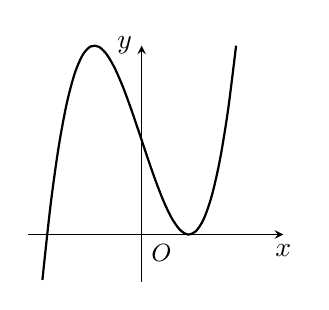
\begin{tikzpicture}[scale=.6]
\draw[-stealth] (-2.4,0) -- (3,0) node[below]{$x$};
\draw[-stealth] (0,-1) -- (0,4) node[left]{$y$};
\draw (0,0) node[below right]{\small $O$};
\draw[thick,smooth] plot[domain=-2.1:2](\x,{(\x)^3-3*(\x)+2});
\end{tikzpicture}
}
\end{ex}

\begin{ex} %{Cau 7}
Cho hàm số $y=f(x)$ có bảng biến thiên như sau:
\\ \centerline{
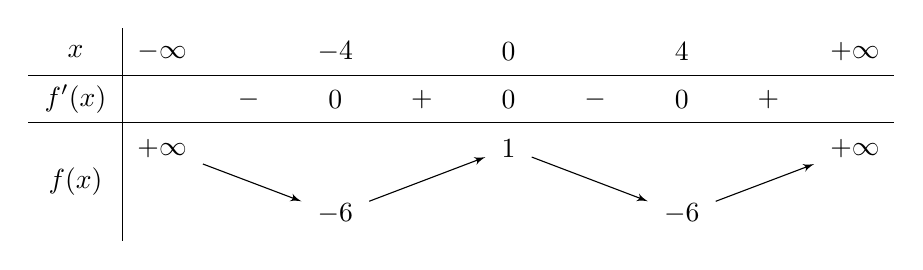
\begin{tikzpicture}
\tkzTabInit[nocadre,lgt=1.2,espcl=2.2]
{$x$ /.6,$f'(x)$ /.6,$f(x)$ /1.5}
{$-\infty$,$-4$,$0$,$4$,$+\infty$}
\tkzTabLine{,-,$0$,+,$0$,-,$0$,+,}
\tkzTabVar{+/ $+\infty$ ,-/$-6$,+/$1$,-/$-6$,+/$+\infty$}
\end{tikzpicture}
}\\
Hàm số đã cho nghịch biến trên khoảng nào dưới đây?
\choice
{$(-6 ; 1)$}
{\True $(0 ; 3)$}
{$(1 ;+\infty)$}
{$(-\infty ;-2)$}
\end{ex}

\begin{ex} %{Cau 8}
Môđun của số phức $z=-1+3 i$ bằng
\choice
{10}
{$\sqrt{2}$}
{\True $\sqrt{10}$}
{2}
\end{ex}

\begin{ex} %{Cau 9}
Thể tích $V$ của khối nón có bán kinh đáy $r$, chiều cao $ h$ được tinh theo công thức nảo đưới đây?
\choice
{\True $V=\frac{1}{3} \pi r^{2} h$}
{$V=\frac{4}{3} \pi r^{2} h$}
{$V=\pi r^{2} h$}
{$V=\frac{2}{3} \pi r^{2} h$}
\end{ex}

\begin{ex} %{Cau 10}
Với$a>0$, biểu thức $\log _{3}(a \sqrt{3})$ bằng
\choice
{\True $\frac{1}{2}+\log _{3} a$}
{$\frac{1}{2} \log _{3} a$}
{$\sqrt{3} \log _{3} a$}
{$\log _{3} a-\frac{1}{2}$}
\end{ex}

\begin{ex} %{Cau 11}
Cho hình lập phương $A B C D \cdot A^{\prime} B^{\prime} C^{\prime} D^{\prime}$. Góc giừa hai đường thẳng $A^{\prime} B$ và $C D$ bằng
\choice
{$30^{\circ}$}
{\True $45^{\circ}$}
{$90^{\circ}$}
{$60^{\circ}$}
\end{ex}

\begin{ex} %{Cau 12}
Trong không gian $Oxyz$, cho hai điểm $A(2 ;-5 ;-3)$ và $B(1 ; 3 ;-1)$. Mặt phằng đi qua $A$ và vuông góc với đường thẳng $A B$ có phương trình là
\choice
{$-x+8 y+2 z-32=0$}
{$-2 x+5 y+3 z+21=0 $}
{\True $-x+8 y+2 z+48=0$}
{$-x+8 y-2 z+16=0$}
\end{ex}

\begin{ex} %{Cau 13}
Trong không gian $Oxyz$, tọa độ tâm của mặt cầu $(S):(x-2)^{2}+(y+1)^{2}+z^{2}=9$ là
\choice
{\True $(2 ;-1 ; 0)$}
{$(1 ; 1 ; 1)$}
{$(2 ;-1 ; 3)$}
{$(-1 ; 2 ; 0)$}
\end{ex}

\begin{ex} %{Cau 14}
Cho các số thực đương $a, b$ thỏa mãn $\log _{3} a+2 \log _{3} b=1$, khằng định nảo dưới đây đúng?
\choice
{$3 a=2 b$}
{\True $a b^{2}=3$}
{$6 a b=1$}
{$a=3 b^{2}$}
\end{ex}

\begin{ex} %{Cau 15}
Cho hàm số $f(x)$ có bảng xét dấu của $f^{\prime}(x)$ như sau
\\ \centerline{
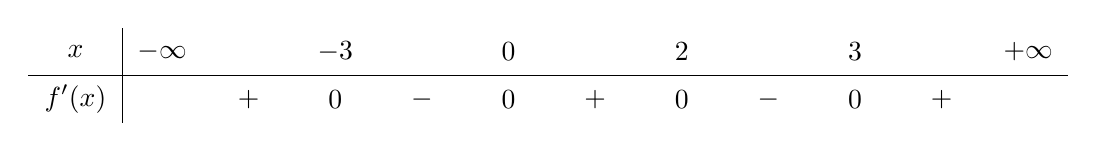
\begin{tikzpicture}
\tkzTabInit[nocadre,lgt=1.2,espcl=2.2]
{$x$ /.6,$f'(x)$ /.6}
{$-\infty$,$-3$,$0$,$2$,$3$,$+\infty$}
\tkzTabLine{,+,$0$,-,$0$,+,$0$,-,$0$,+,}
\end{tikzpicture}
}\\
Số điểm cực trị của hàm số đã cho là
\choice
{$1$}
{$3$}
{\True $4$ }
{$2$}
\end{ex}

\begin{ex} %{Cau 16}
Tiệm cận ngang của đồ thị hàm số $y=\dfrac{2x+3}{x-1} $ là đường thẳng có phương trình
\choice
{\True $y=2$}
{$y=3$}
{$x=1$}
{$y=-3$}
\end{ex}

\begin{ex} %{Cau 17}
Nghiệm của phương trình$ \log_2{x-1}=3$ là
\choice
{$x=7$}
{$x=4$}
{\True$x=9$}
{$x=3$}
\end{ex}

\begin{ex} %{Cau 18}
\immini[thm]{Cho hàm số $y=a x^3+b x^2+c x+d\quad (a, b, c, d \in \mathbb{R})$ có đồ thị là đường
 cong trong hình bên. Giá trị cực tiểu của hàm số đã cho bằng
\choice
{$0$}
{$1$}
{$3$}
{\True $-1$}
}{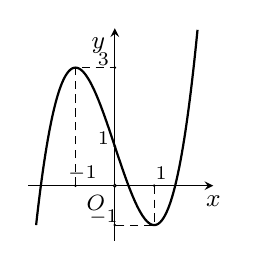
\begin{tikzpicture}[scale=.5]
\draw[-stealth] (-2.2,0) -- (2.5,0) node[below]{\small $x$};
\draw[-stealth] (0,-1.4) -- (0,4) node[below left]{\small $y$};
\draw [thin,densely dashed] (-1,0)|-(0,3) (1,0)|-(0,-1);
\draw[thick,smooth,samples=100] plot[domain=-2:2.1](\x,{(\x)^3-3*(\x)+1});
\draw [fill=white,draw=black] (0,0) circle (1pt)node[below left]{\footnotesize $O$};
\foreach \x in{-1,1}\draw(\x,0) circle (.5pt) node[shift={(60:5pt)}]{\scriptsize $\x$};
\foreach \y in{-1,1,3}\draw(0,\y) circle (.5pt) node[shift={(145:5pt)}]{\scriptsize $\y$};
\end{tikzpicture}}
\end{ex}

\begin{ex} %{Cau 19}
Cho số phức $z=-2+3 i$, khi đó $3 z$ bằng 
\choice
{$-6+3i$}
{\True $-6+9i$}
{$6-9i$}
{$-2+9i$}
\end{ex}

\begin{ex} %{Cau 20}
Nếu $\int_{-2}^{3} f(x) \mathrm{d} x=-2$  thì $\int_{-2}^{3} 3 f(x) \mathrm{d} x$ bằng 
\choice
{$3$}
{\True$-6$}
{$1$}
{$-5$}
\end{ex}

\begin{ex} %{Cau 21}
Trong các hàm số đưới đây, hàm số nào không có cực trị ?
\choice
{$y=-3 x^{3}+2 x$}
{$y=3 x^{3}-2 x$}
{$y=2 x^{3}-x$}
{\True$y=-2 x^{3}-3 x$}
\end{ex}

\begin{ex} %{Cau 22}
Trên khoảng $(0 ;+\infty)$ họ nguyên hàm của hàm số $f(x)=\sqrt[3]{x}$ là
\choice
{$\int f(x) ~\mathrm{d} x=3 x^{\frac{1}{3}}+C$}
{$\int f(x) ~\mathrm{d} x=\frac{1}{3} x^{\frac{1}{3}}+C$}
{$\int f(x) ~\mathrm{d} x=\frac{1}{4} x^{\frac{4}{3}}+C$}
{\True$\int f(x) ~\mathrm{d} x=\frac{3}{4} x^{\frac{4}{3}}+C$}
\end{ex}

\begin{ex} %{Cau 23}
Giao điểm của đồ thị hàm số $y=-3 x^{3}+5 x-2$ với truc tung có tọa độ là
\choice
{$(1 ; 0)$}
{$\left(\frac{2}{3} ; 0\right)$}
{$\left(0 ; \frac{2}{3}\right)$}
{\True $(0 ;-2)$}
\end{ex}

\begin{ex} %{Cau 24}
Cho hàm số $f(x)=2 x-3 \sin x$. Khẳng định nào dưới đây đúng ?
\choice
{$\int f(x) ~\mathrm{d} x=x^{2}-3 \cos x+ C $}
{\True $\int f(x) ~\mathrm{d} x=x^{2}+3 \cos x+ C $}
{$\int f(x) ~\mathrm{d} x=2-3 \cos x+ C $}
{$\int f(x) ~\mathrm{d} x=2+3 \cos x+ C $}
\end{ex}

\begin{ex} %{Cau 25}
Cho khối lăng tru có điện tích đáy bẳng $5$ và chiều cao bằng$ 3$ . Thể tích của khối lãng trụ đã cho bằng
\choice
{$24$}
{$45$}
{\True $15$}
{$5$}
\end{ex}
\begin{ex} %{Cau 26}
Trến mặt phẳng tọa độ, cho $M(-3 ; 1)$ là điểm biều diễn của số phức $z$. Phần thực của $z$ bằng
\choice
{\True$-3$}
{$1$}
{$3$}
{$-1$}
\end{ex}
\begin{ex} %{Cau 27}
Trong không gian $O x y z$, cho hai vectơ $\vec{a}=(-1 ; 3 ;-3)$ và $\vec{b}=(2 ; 1 ;-2)$. Tọa độ của vecto $\vec{b}-\vec{a}$ là
\choice
{\True $(3 ;-2 ; 1)$}
{$(1 ; 4 ;-5)$}
{$(1 ;-2 ; 3)$}
{$(3 ; 2 ;-1)$}
\end{ex}
\begin{ex} %{Cau 28}
Điểm nào dưói đây \textbf{không} thuộc đồ thị hảm số $y=x^{4}-x^{2}-5$ ?
\choice
{$(1;-5)$}
{$(-1;-5)$}
{\True$(-2;6)$}
{$(2;7)$}
\end{ex}
\begin{ex} %{Cau 29}
Trong không gian $O x y z$,  đường thẳng $ d: \frac{x+1}{2}=\frac{y-2}{-1}=\frac{z}{3}$  đi qua điêm nào dưới đây?
\choice
{$A(2 ;-1 ; 3)$}
{\True $C(-1 ; 2 ; 0)$}
{$B(0 ; 2 ;-1)$}
{$D(1 ;-2 ; 0)$}
\end{ex}
\begin{ex} %{Cau 30}
Nếu $\int_{1}^{2} f(x) ~\mathrm{d} x=3$ và $\int^{2} g(x) ~\mathrm{d} x=-2$ thì $\int^{2}[f(x)-g(x)] ~\mathrm{d} x$ bằng
\choice
{$1$}
{\True $5$}
{$-5$}
{$6$}
\end{ex}
\begin{ex} %{Cau 31}
Trong không gian $Oxyz$, mặt phẳng $(P):x-4 y+5 z-2=0$ có một vectơ pháp tuyến là:
\choice
{$\overrightarrow{u_{1}}=(-1 ; 4 ; 5)$}
{\True $\overrightarrow{u_{2}}=(1 ;- 4 ; 5)$}
{$\overrightarrow{u_{3}}=(5 ; -4 ; 1)$}
{$\overrightarrow{u_{4}}=(-4 ; 5 ; -2)$}
\end{ex}
\begin{ex} %{Cau 32}
Trên đoạn $\left[\frac{1}{3} ; \frac{3}{2}\right]$, hàm số $y=2 x^{2}+\frac{1}{2 x}$ đạt giá trị nhỏ nhất tại điểm
\choice
{$x=\frac{1}{2}$}
{\True$x=\frac{3}{2}$}
{$x=1$}
{$x=\frac{1}{3}$}
\end{ex}
\begin{ex} %{Cau 33}
Tập xác định của hàm số $y=x^{\sqrt{5}}$ là
\choice
{\True$(0 ;+\infty)$}
{$\mathbb{R}$}
{$\mathbb{R} \backslash\{0\}$}
{$(5 ;+\infty)$}
\end{ex}
\begin{ex} %{Cau 34}
Trên khoảng $(0 ;+\infty)$, đạo hàm của hàm số $y=\log _{\sqrt{3}} x$ là
\choice
{$y^{\prime}=\frac{1}{2 x \ln \sqrt{3}}$}
{$y^{\prime}=\frac{\sqrt{3}}{x \ln 3}$}
{$y^{\prime}=\frac{\sqrt[3]{3}}{x}$}
{\True$y^{\prime}=\frac{1}{x \ln \sqrt{3}}$}
\end{ex}
\begin{ex} %{Cau 35}
Nếu $\int_{-1}^{2} f(x) \mathrm{d} x=3$ thì $\int_{-1}^{2}[f(x)-4 x] \mathrm{d} x$ bằng
\choice
{$1 $}
{$4$}
{$-5$}
{\True $-3$}
\end{ex}
\begin{ex} %{Cau 36}
Gọi $z_{1}, z_{2}$ là các nghiệm phức của phương trình $z^{2}-2 z+17=0$. Giá trị của biểu thức $3\left(z_{1}+z_{2}\right)-z_{1} z_{2}$ bằng 
\choice
{\True $-11$}
{$23$}
{$16$}
{$-8$}
\end{ex}
\begin{ex} %{Cau 37}
Cho hinh nón đỉnh $S$, đường tròn đáy có tâm $O$ và góc ở đỉnh bẳng $120^{\circ}$. Một mặt phẳng đi qua $S$ cắt hình nón theo thiết diện là tam giác vuông $S A B$. Biết khoảng cách giữa hai đường thẳng $A B$ và $S O$ bằng 3 , diện tích xung quanh của hinh nón đã cho bằng
\choice
{$12 \pi \sqrt{3}$}
{$27 \pi \sqrt{3}$}
{\True $18 \pi \sqrt{3}$}
{$9 \pi \sqrt{3}$}
\end{ex}

\begin{ex} %{Cau 38}
Số giao điểm của đồ thị hàm số $y=x^3+4x^2-11x-30$ với trục hoành là 
\choice 
{ $0$}
{ $1$}
{ $2$}
{\True $3$} 
\end{ex} 
\begin{ex} %{Cau 39}
Trong không gian $Oxyz$, cho điểm $A( 3;\,1;\,-2 )$. Đường thẳng đi qua $A$ và song song với đường thẳng\\ $\Delta:\dfrac{x}{2}=\dfrac{y+1}{-1}=\dfrac{z-2}{1}$ có phương trình là
\choice 
{\True $\heva{
& x=3+2t \\ 
& y=1-t \\ 
& z=-2+t \\ 
}$}
{ $\heva{
& x=2+3t \\ 
& y=-1+t \\ 
& z=1-2t \\ 
}$}
{ $\heva{
& x=-3+2t \\ 
& y=-1-t \\ 
& z=2+t \\ 
}$}
{ $\heva{
& x=3-2\,t \\ 
& y=1+t \\ 
& z=-2+t \\ 
}$} 
\end{ex} 

\begin{ex} %{Cau 40}
Trong không gian $Oxyz$, cho điểm $A( 1;1;2 )$ và hai đường thẳng ${{d}_{1}}:\heva{
& x=3+t \\ 
& y=-1+2t \\ 
& z=4 \\ 
}$ và ${{d}_{2}}:\dfrac{x+2}{1}=\dfrac{y}{1}=\dfrac{z-2}{2}$. Đường thẳng qua $A$, cắt đường thẳng ${{d}_{1}},{{d}_{2}}$ có phương trình là
\choice 
{ $\dfrac{x-1}{1}=\dfrac{y-1}{1}=\dfrac{z-2}{-1}$}
{ $\dfrac{x-1}{1}=\dfrac{y-1}{-1}=\dfrac{z-2}{1}$} 
{\True $\dfrac{x-1}{2}=\dfrac{y-1}{1}=\dfrac{z-2}{1}$}
{ $\dfrac{x-1}{1}=\dfrac{y-1}{2}=\dfrac{z-2}{-1}$} 
\end{ex} 
\begin{ex} %{Cau 41}
Trên tập hợp các số phức, cho phương trình ${{z}^2}+az+b=0,\,\,( a,\,b\in \mathbb{R} )$. Biết phương trình đã cho có hai nghiệm là ${{z}_{1}}=2-i$ và ${{z}_{2}}$, khi đó giá trị của $\bigg| a{{z}_{1}}-b{{z}_{2}} \bigg|$ bằng 
\choice 
{ $6\sqrt{10}$}
{ $18$}
{ $15\sqrt{3}$}
{\True $5\sqrt{13}$} 
\end{ex} 
\begin{ex} %{Cau 42}
Cho hai hàm số $f( x )=ax^3+bx^2+cx-4$ và $g( x )=dx^2+ex+2,\ ( a,\ b,\ c,\ d,\ e\in \mathbb{R} )$. Biết rằng đồ thị hàm số $y=f( x )$ và $y=g( x )$ cắt nhau tại $3$ điểm có hoành độ lần lượt là $-3;\ -1;\ 2$. Hình phẳng giới hạn bởi đồ thị hai hàm số đã cho có diện tích bằng.
\choice 
{ $\dfrac{316}{15}$}
{ $\dfrac{191}{9}$}
{ \True $\dfrac{253}{12}$}
{ $\dfrac{97}{6}$} 
\end{ex}
\Closesolutionfile{ans}
\begin{name}
{Sở GD Nam Định}
{ĐỀ THI THỬ TỐT NGHIỆP THPT--NĂM 2022 }
\end{name}
\Opensolutionfile{ans}[sonamdinh-]

\begin{ex} 
 Môđun của số phức $z=4+2 i$ bằng
\choice 
 { 20 } 
 { 6 } 
 { $2 \sqrt{5}$} 
 { 8 }
\end{ex} 
 
\begin{ex} 
 Trong không gian $O x y z$, mặt cầu $(S):(x-2)^{2}+(y-2)^{2}+(z+1)^{2}=16$ có bán kính bằng
\choice 
 { 4 } 
 { 16 } 
 { 2 } 
 { 9 }
\end{ex} 
 
\begin{ex} 
 Điểm nào dưới đây thuộc đồ thị của hàm số $y=2 x^{4}-x^{2}-1$ ?
\choice 
 { $E(-1 ; 0)$} 
 { $F(-1 ; 2)$} 
 { $K(-1 ; 4)$} 
 { $D(-1 ; 1)$}
\end{ex} 
 
\begin{ex} 
 Diện tích $S$ của mặt cầu bán kính $r$ được tính theo công thức nào dưới đây?
\choice 
 { $S=\pi r^{2}$} 
 { $S=\frac{4}{3} \pi r^{2}$} 
 { $S=2 \pi r^{2}$} 
 { $S=4 \pi r^{2}$}
\end{ex} 
 
\begin{ex} 
 Trên khoảng $(-\infty ;+\infty)$, họ nguyên hàm của hàm số $f(x)=5^{x}$ là
\choice 
 { $5^{x} \ln 5+C$} 
 { $\frac{5^{x}}{\ln 5}+C$} 
 { $5^{x}+C$} 
 { $\frac{5^{x+1}}{x+1}+C$}
\end{ex} 
 
\begin{ex} 
 Cho hàm số $f(x)$ có bảng xét dấu của đạo hàm như sau:
\\ \centerline{
\begin{tikzpicture}
\tkzTabInit[nocadre,lgt=1.2,espcl=2.2]
{$x$ /.6,$f'(x)$ /.6}
{$-\infty$,$1$,$2$,$3$,$4$,$+\infty$}
\tkzTabLine{,-,$0$,+,$0$,+,$0$,-,$0$,+,}
%\tkzTabVar{-/ $-\infty$ ,+/$3$,-/$-1$,+/$3$,-/$-\infty$}
\end{tikzpicture}
}\\
Số điểm cực trị của hàm số đã cho là
\choice 
 { 4 } 
 { 3 } 
 { 2 } 
 { 5 }
\end{ex} 
 
\begin{ex} 
 Tập nghiệm của bất phương trình $\left(\frac{1}{2}\right)^{x}>1$ là
\choice 
 { $(0 ;+\infty)$} 
 { $\mathbb{R}$} 
 { $(-\infty ; 0)$} 
 { $(2 ;+\infty)$}
\end{ex} 
 
\begin{ex} 
 Cho khối chóp có diện tích đáy $B=6$ và chiều cao $h=7$. Thể tích của khối chóp đã cho bằng
\choice 
 { 42 } 
 { 126 } 
 { 14} 
 { 56 }
\end{ex} 
 
\begin{ex} 
 Tập xác định của hàm số $y=x^{\sqrt{3}}$ là
\choice 
 { $\mathbb{R}$} 
 { $(0 ;+\infty)$} 
 { $\mathbb{R} \backslash\{0\}$} 
 { $[0 ;+\infty)$}
\end{ex} 
 
\begin{ex} 
 Nghiệm của phương trình $\log _{3}(x+5)=2$ là
\choice 
 { $x=4$} 
 { $x=3$} 
 { $x=1$} 
 { $x=-3$}
\end{ex} 
 
\begin{ex} 
 Nếu $\int_{0}^{1} f(x) d x=2$ và $\int_{0}^{1} g(x) d x=-3$ thì $\int_{0}^{1}[2 f(x)+g(x)] d x$ bằng
\choice 
 { 7 } 
 { $-1$} 
 { $-4$} 
 { 1 }
\end{ex} 
 
\begin{ex} 
 Cho số phức $z_{1}=2+3 i$ và số phức $z_{2}=3-2 i$. Phần thực của số phức $z_{1}+z_{2}$ bằng
\choice 
 { 1 } 
 { 0 } 
 { 5 } 
 { $\sqrt{13}$}
\end{ex} 
 
\begin{ex} 
 Trong không gian $O x y z$, cho mặt phẳng $(\alpha): x-2 y+3 z-4=0$. Vectơ nào dưới đây là một vectơ pháp tuyến của mặt phẳng $(\alpha)$ ?
\choice 
 { $\overrightarrow{n_{2}}=(1 ;-2 ; 3)$} 
 { $\vec{n}_{1}=(1 ; 2 ; 3)$} 
 { $\overrightarrow{n_{4}}=(-2 ; 3 ;-4)$} 
 { $\overrightarrow{n_{3}}=(1 ; 3 ; 4)$}
\end{ex} 
 
\begin{ex} 
 Trong không gian $O x y z$, cho hai vectơ $\vec{a}=(1 ; 3 ; 2)$ và $\vec{b}=(3 ; 1 ; 2)$. Tọa độ của vectơ $\vec{a}+2 \vec{b}$ là
\choice 
 { $(7 ; 4 ; 4)$} 
 { $(7 ; 5 ; 6)$} 
 { $(5 ; 5 ; 4)$} 
 { $(4 ; 4 ; 4)$}
\end{ex} 
 
\begin{ex} 
 Trong mặt phẳng tọa độ $O x y$, cho $M(2 ;-3)$ là điểm biểu diễn số phức $z$. Phần ảo của số phức $z$ là
\choice 
 { $\sqrt{13}$} 
 { 2 } 
 { $-3 i$} 
 { $-3$}
\end{ex} 
 
\begin{ex} 
 Tiệm cận ngang của đồ thị hàm số $y=\frac{3 x-2}{x+2}$ là đường thẳng có phương trình:
\choice 
 { $y=3$} 
 { $y=-2$} 
 { $y=-1$} 
 { $y=-3$}
\end{ex} 
 
\begin{ex} 
 Với mọi số thực dương $x, \log _{3}\left(\frac{x^{3}}{3}\right)$ bằng
\choice 
 { $3 \log _{3} x-1$} 
 { $\log _{3} x-1$} 
 { $\log _{3} x$} 
 { $3 \log _{3} x+1$}
\end{ex} 
 
\begin{ex} 
 \immini[thm]{Hàm số nào dưới đây có đồ thị như đường cong trong hình vẽ bên?
\choice 
 { $y=x^{2}-2 x-2$} 
 { $y=x^{3}-3 x-2$} 
 { $y=x^{4}-4 x^{2}+2$} 
 { $y=-x^{4}+4 x^{2}+2$}}
 {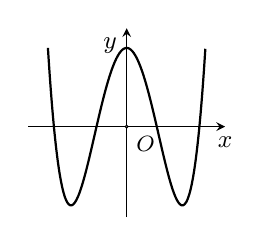
\begin{tikzpicture}[scale=.5]
\draw[-stealth] (-2.5,0) -- (2.5,0) node[below]{\small $x$};
\draw[-stealth] (0,-2.3) -- (0,2.5) node[below left]{\small $y$};
\draw[thick,smooth,samples=100] plot[domain=-2:2](\x,{(\x)^4-4*(\x)^2+2});
\draw [fill=white,draw=black] (0,0) circle (1pt)node[below right]{\footnotesize $O$};
\end{tikzpicture}
 }
\end{ex} 
 
\begin{ex} 
 Trong không gian $O x y z$, cho đường thẳng $d:\left\{\begin{array}{l}x=1-2 t y=3+t z=-1-t\end{array}\right.$. Đường thẳng $d$ đi qua điểm nào dưới đây?
\choice 
 { $E(5 ; 1 ; 1)$} 
 { $H(1 ; 3 ; 1)$} 
 { $T(-2 ; 1 ;-1)$} 
 { $Q(-5 ; 0 ; 1)$}
\end{ex} 
 
\begin{ex} 
 Với $n$ là số nguyên dương và $k$ là số tự nhiên, $k \leq n$, công thức nào dưới đây đúng?
\choice 
 { $A_{n}^{k}=\frac{n !}{k !}$} 
 { $C_{n}^{k}=\frac{n !}{(n-k) !}$} 
 { $A_{n}^{k}=\frac{n !}{(n-k) !}$} 
 { $C_{n}^{k}=\frac{(n-k) ! k !}{n !}$}
\end{ex} 
 
\begin{ex} 
 Cho khối hộp có diện tích đáy là $B$ và chiều cao là $h$. Thể tích $V$ của khối hộp này là
\choice 
 { $V=\frac{1}{3} B h$} 
 { $V=B h$} 
 { $V=2 B h$} 
 { $V=\frac{1}{6} B h$}
\end{ex} 
 
\begin{ex} 
 Trên khoảng $(0 ;+\infty)$, đạo hàm của hàm số $y=\log _{\frac{1}{3}} x$ là
\choice 
 { $y^{\prime}=\frac{1}{x \ln 3}$} 
 { $y^{\prime}=-\frac{1}{x \ln 3}$} 
 { $y^{\prime}=-\frac{\ln 3}{x}$} 
 { $y^{\prime}=\frac{1}{x}$}
\end{ex} 
 
\begin{ex} 
 Cho hàm số $f(x)$ có bảng biến thiên như sau
\\ \centerline{
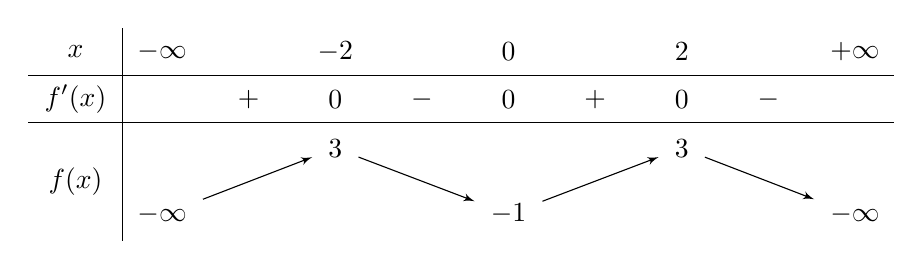
\begin{tikzpicture}
\tkzTabInit[nocadre,lgt=1.2,espcl=2.2]
{$x$ /.6,$f'(x)$ /.6,$f(x)$ /1.5}
{$-\infty$,$-2$,$0$,$2$,$+\infty$}
\tkzTabLine{,+,$0$,-,$0$,+,$0$,-,}
\tkzTabVar{-/ $-\infty$ ,+/$3$,-/$-1$,+/$3$,-/$-\infty$}
\end{tikzpicture}
}\\
Hàm số $f(x)$ nghịch biến trên khoảng nào dưới đây?
\choice 
 { $(-\infty ; 3)$} 
 { $(-2 ; 2)$} 
 { $(-2 ; 0)$} 
 { $(-1 ; 3)$}
\end{ex} 
 
\begin{ex} 
 Cho khối trụ có bán kính đáy bằng $r$ và độ dài đường sinh bằng $l$. Thể tích của khối trụ đã cho bằng
\choice 
 { $\frac{1}{3} \pi r^{2} l$} 
 { $\pi r^{2} l$} 
 { $2 \pi r^{2} l$} 
 { $\frac{1}{2} \pi r^{2} l$}
\end{ex} 
 
\begin{ex} 
 Nếu $\int_{1}^{3} f(x) d x=2$ và $\int_{3}^{5} f(x) d x=-2$ thì $\int_{1}^{5} f(x) d x$ bằng
\choice 
 { 0 } 
 { 4 } 
 { $-4$} 
 { 2 }
\end{ex} 
 
\begin{ex} 
 Cho cấp số nhân $\left(u_{n}\right)$ có $u_{2}=2$ và $u_{3}=6$. Tìm công bội $q$ của cấp số nhân đã cho.
\choice 
 { $q=3$} 
 { $q=4$} 
 { $q=8$} 
 { $q=12$}
\end{ex} 
 
\begin{ex} 
 Cho hàm số $f(x)=\cos x-1$. Khẳng định nào dưới đây là đúng?
\choice 
 { $\int f(x) d x=-\sin x-x+C$} 
 { $\int f(x) d x=-\sin x+C$} 
 { $\int f(x) d x=\sin x-x+C$} 
 { $\int f(x) d x=\sin x+x+C$}
\end{ex} 
 
\begin{ex} 
 \immini[thm]{Cho hàm số $y=a x^{3}+b x^{2}+c x+d$ (với $a, b, c, d \in \mathbb{R}$ và $a \neq 0$ ) có đồ thị là đường cong trong hình bên. Giá trị cực đại của hàm số đã cho bằng
\choice 
 { 2 } 
 { 1 } 
 { $-1$} 
 { $-2$}}
 {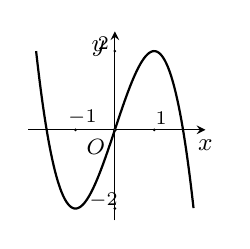
\begin{tikzpicture}[scale=.5]
\draw[-stealth] (-2.2,0) -- (2.3,0) node[below]{\small $x$};
\draw[-stealth] (0,-2.3) -- (0,2.5) node[below left]{\small $y$};
\draw[thick,smooth,samples=100] plot[domain=-2:2](\x,{-(\x)^3+3*(\x)});
\draw [fill=white,draw=black] (0,0) circle (1pt)node[below left]{\footnotesize $O$};
\foreach \x in{-1,1}\draw(\x,0) circle (.5pt) node[shift={(60:5pt)}]{\scriptsize $\x$};
\foreach \y in{-2,2}\draw(0,\y) circle (.5pt) node[shift={(145:5pt)}]{\scriptsize $\y$};
\end{tikzpicture}}
\end{ex} 
 
\begin{ex} 
 Trên đoạn $[1 ; 6]$, hàm số $y=x+\frac{9}{x+1}$ đạt giá trị nhỏ nhất tại điểm
\choice 
 { $x=1$} 
 { $x=8$} 
 { $x=2$} 
 { $x=6$}
\end{ex} 
 
\begin{ex} 
 Hàm số nào dưới đây đồng biến trên $(-\infty ;+\infty)$ ? 
 \choice 
{ $y=x^{3}+3 x-1$} 
 { $y=\frac{x}{x+2}$}
{ $y=x^{2}+1$} 
 { $y=x^{4}-2 x^{2}$}
\end{ex} 
 
\begin{ex} 
 Với mọi $a, b$ thỏa mãn $2 \log _{9} a-3 \log _{3} b=1$, mệnh đề nào dưới đây đúng?
\choice 
 { $a=\frac{3}{b^{3}}$} 
 { $2 a-3 b=1$} 
 { $a^{2}=3 b^{3}$} 
 { $a=3 b^{3}$}
\end{ex} 
 
\begin{ex} 
 Cho hình lập phương $A B C D \cdot A^{\prime} B^{\prime} C^{\prime} D^{\prime}$. Góc giữa hai đường thẳng $B A^{\prime}$ và $C C^{\prime}$ bằng
\choice 
 { $90^{0}$} 
 { $60^{0}$} 
 { $45^{0}$} 
 { $30^{0}$}
\end{ex} 
 
\begin{ex} 
 Nếu $\int_{2}^{4} f(x) d x=3$ thì $\int_{2}^{4}\left[f(x)-x^{3}\right] d x$ bằng
\choice 
 { $-57$} 
 { 63 } 
 { $-33$} 
 { $-237$}
\end{ex} 
 
\begin{ex} 
 Trong không gian $O x y z$, cho điểm $M(1 ;-2 ; 3)$ và mặt phẳng $(P): 2 x+y+z-1=0$. Đường thẳng đi qua điểm $M$ và vuông góc với mặt phẳng $(P)$ có phương trình là
 \choice
{ $\frac{x+2}{1}=\frac{y+1}{-2}=\frac{z+1}{3}$}
 { $\frac{x+1}{2}=\frac{y-2}{1}=\frac{z+3}{1}$} 
 { $\frac{x-1}{2}=\frac{y+2}{1}=\frac{z-3}{1}$} 
 { $\frac{x-2}{1}=\frac{y-1}{-2}=\frac{z-1}{3}$}
\end{ex} 
 
\begin{ex} 
 Cho số phức $z$ thỏa mãn $(1+i)(z-2)=4 i$. Phần ảo của số phức $\bar{z}$ bằng
\choice 
 { 4 } 
 { $-4$} 
 { 2 } 
 { $-2$}
\end{ex} 
 
 
\begin{ex} 
 Trong hộp có 30 tấm thẻ được đánh số thứ tự lần lượt từ số 1 đến số 30 . Người ta lấy ngẫu nhiên cùng một lúc từ hộp ra hai tấm thẻ rồi nhân số thứ tự của hai thẻ lấy được với nhau. Tính xác suất để tích thu được là một số chẵn.
\choice 
 { $\frac{1}{2}$} 
 { $\frac{22}{29}$} 
 { $\frac{7}{29}$} 
 { $\frac{51}{58}$}
\end{ex} 
 
\begin{ex} 
 Trong không gian $O x y z$, cho tứ diện $A B C D$ với $A=(2 ; 1 ; 2), B=(3 ; 2 ; 0), C=(1 ; 1 ; 3)$, $D=(-2 ; 2 ; 4)$. Mặt phẳng đi qua $D$ và song song với mặt phẳng $(A B C)$ có phương trình là
\choice 
 { $3 x-y+z+4=0$} 
 { $3 x+y+z=0$} 
 { $x+y+z-4=0$} 
 { $x-y+z=0$}
\end{ex} 
 
 \begin{ex} 
 Cho hình lăng trụ tam giác đều $A B C \cdot A^{\prime} B^{\prime} C^{\prime}$ với $A B=2$ và
$A A^{\prime}=3$. Tính khoảng cách $d$ từ điểm $A$ đến mặt phẳng $\left(A^{\prime} B C\right)$.
\choice 
 { $d=\frac{3}{2}$} 
 { $d=\frac{2}{3}$} 
 { $d=\frac{3}{\sqrt{13}}$} 
 { $d=\frac{6}{\sqrt{13}}$}
\end{ex} 

\begin{ex} 
 Cho hàm số đa thức bậc ba $y=f(x)$ có bảng biến thiên như sau:
\\ \centerline{
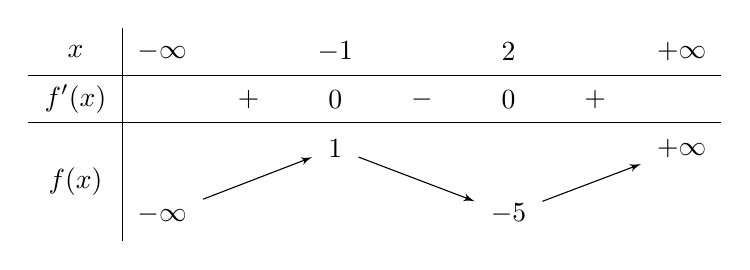
\begin{tikzpicture}
\tkzTabInit[nocadre,lgt=1.2,espcl=2.2]
{$x$ /.6,$f'(x)$ /.6,$f(x)$ /1.5}
{$-\infty$,$-1$,$2$,$+\infty$}
\tkzTabLine{,+,$0$,-,$0$,+,}
\tkzTabVar{-/ $-\infty$ ,+/$1$,-/$-5$,+/$+\infty$}
\end{tikzpicture}
}\\
Có bao nhiêu giá trị nguyên của tham số $m$ để phương trình $f^{\prime}(f(x)+m)=0$ có đúng bốn nghiệm thực phân biệt?
\choice
 { 4 } 
 { 5 } 
 { 0}
 { 6 }
\end{ex} 
 
\begin{ex} 
 Cho hàm số $y=f(x)$ có đạo hàm $f^{\prime}(x)$ thoả mãn $\left(1+x^{2}\right) f^{\prime}(x)-1=3 x^{4}+4 x^{2}, \forall x \in \mathbb{R}$ và $f(1)=0$. Biết $F(x)$ là một nguyên hàm của hàm số $21 . f\left(x^{2}\right)$ và $F(0)=10$, hãy tính $F(2)$
\choice
 { $F(2)=\frac{566}{21}$}
 { $F(2)=566$} 
 { $F(2)=366$} 
 { $F(2)=52$}
\end{ex} 
 
\begin{ex} 
 Cho khối chóp $S . A B C D$ có $S A \perp(A B C D)$. Đáy $A B C D$ là hình chữ nhật với $A B=a \sqrt{3}, A D=a$. Biết góc giữa hai mặt phẳng $(S A B)$ và $(S B D)$ bằng $45^{\circ}$, hãy tính theo $a$ thể tích $V$ của khối chóp $S . A B C D$ 
 \choice 
{ $V=\frac{\sqrt{2}}{2} a^{3}$} 
 { $V=\frac{\sqrt{2}}{6} a^{3}$}
{ $V=\frac{\sqrt{6}}{6} a^{3}$} 
 { $V=3 \sqrt{2} a^{3}$}
\end{ex} 
 
\begin{ex} 
 Trên tập hợp số phức, xét phương trình $z^{2}-2 z+m-3=0$ (với $m$ là tham số thực). Gọi hai điểm $A$ và $B$ là hai điểm biểu diễn hai nghiệm của phương trình đã cho. Biết rằng ba điểm $O, A, B$ là ba đỉnh của một tam giác vuông (với $O$ là gốc tọa độ), khẳng định nào dưới đây đúng?
\choice 
 { $m \in[3 ; 8)$} 
 { $m \in(-2 ; 3)$} 
 { $m \in[8 ; 10]$} 
 { $m \in(-6 ;-2]$}
\end{ex} 
 
\begin{ex} 
 Xét hai số phức $z_{1}, z_{2}$ thoả mãn $\left|z_{1}-3-5 i\right|=2$ và $\left|z_{2}+3+3 i\right|=3$. Gọi $M, m$ lần lượt là giá trị lớn nhất và giá trị nhỏ nhất của $\left|z_{1}-z_{2}\right|$, khi đó $M+m$ bằng
\choice 
 { 25 } 
 { 15 } 
 { 10 } 
 { 20 }
\end{ex} 
 
\begin{ex} 
 Cho khối nón đỉnh $S$ có đáy là hình tròn tâm $O$. Gọi $A$ và $B$ là hai điểm thuộc đường tròn đáy sao cho tam giác $S A B$ vuông và có diện tích bằng 16 . Góc tạo bởi giữa trục $S O$ và mặt phẳng $(S A B)$ bằng $30^{\circ}$. Thể tích của khối nón đã cho bằng
 \choice
{ $\frac{40 \sqrt{2}}{3} \pi$} 
 { $\frac{10 \sqrt{6}}{3} \pi$} 
 { $\frac{20 \sqrt{3}}{3} \pi$}
 { $\frac{40 \sqrt{3}}{3} \pi$}
\end{ex} 
 
\Closesolutionfile{ans}
\end{document}
